\documentclass[conference]{IEEEtran}
\IEEEoverridecommandlockouts
% The preceding line is only needed to identify funding in the first footnote. If that is unneeded, please comment it out.
\usepackage{cite}
\usepackage{amsmath,amssymb,amsfonts}
\usepackage{algorithmic}
\usepackage{graphicx}
\usepackage{textcomp}
\usepackage{xcolor}
\usepackage[utf8]{inputenc} % usually not needed (loaded by default)
\usepackage[T1]{fontenc}
\def\BibTeX{{\rm B\kern-.05em{\sc i\kern-.025em b}\kern-.08em
    T\kern-.1667em\lower.7ex\hbox{E}\kern-.125emX}}
\begin{document}

\title{Predição de Fluxo de Veículos em Cruzamentos: Comparando os Algoritmos Tradicionais com Deep Learning}

\author{\IEEEauthorblockN{Claudio S. R. Silva Filho}
\IEEEauthorblockA{\textit{Laboratório de Transporte} \\
\textit{Universidade de Brasília}\\
Brasília, Brasil \\
claudiosegalafilho@gmail.com}
\and
\IEEEauthorblockN{Pedro Henrique S. Gonzaga}
\IEEEauthorblockA{\textit{Laboratório de Transporte} \\
\textit{Universidade de Brasília}\\
Brasília, Brasil \\
pgonzaga095@gmail.com}
\and
\IEEEauthorblockN{Li Weigang}
\IEEEauthorblockA{\textit{Laboratório de Transporte} \\
\textit{Universidade de Brasília}\\
Brasília, Brasil \\
weigangbr@gmail.com}
\and
\IEEEauthorblockN{Geraldo Pereira}
\IEEEauthorblockA{\textit{Laboratório de Transporte} \\
\textit{Universidade de Brasília}\\
Brasília, Brasil \\
geraldoprfilho@gmail.com}
}

\maketitle

\begin{abstract}
Predição de fluxo de veículos é uma tarefa complexa com vários fatores desafiadores como a escalabilidade, a oscilação do fluxo e os fatores randômicos. A literatura, em sua maioria, foca em vias livres. Visto isso, este artigo aborda cinco modelos de aprendizagem de máquina comumente usados para resolver o problema com vias livres (\textit{Long Short Term Memory Neural Network}, \textit{Gated Recurrent Unit Neural Network}, \textit{Recurrent Neural Network}, \textit{Support Vector Machine} e \textit{Random Forest}) para verificar se os modelos conseguem ter uma performance satisfatória em vias urbanas, mais especificamente cruzamentos. Esta pesquisa ainda está em andamento, mas os modelos já se mostraram significativamente superiores que as bases de comparação.
\end{abstract}

\begin{IEEEkeywords}
cruzamento, aprendizagem de máquina, predição de fluxo, redes neurais, veículos, trânsito, tráfego
\end{IEEEkeywords}

\section{Introdução}

O volume de carros tem aumentado ao longo dos últimos anos e as vias públicas não tem conseguido acompanhar este crescimento \cite{b7}. Com isso, os congestionamentos tendem a piorar, aumentando a emissão de gases poluentes na atmosfera, poluição sonora e o tempo gasto pelos motoristas no trânsito, diminuindo assim a qualidade de vida do habitantes de uma cidade.

Um dos meios de amenizar o congestionamento é tentar prever quando ele irá acontecer. Uma vez que os cidadãos saibam que um engarrafamento irá ocorrer, eles podem se planejar melhor e tomar rotas alternativas, distribuindo melhor os carros na malha viária. Já organizações governamentais poderiam usar os dados para ter uma noção em tempo real de como está o fluxo pela cidade, podendo agir antes de um engarrafamento acontecer.

A literatura está saturada com artigos de predição de fluxo utilizando aprendizagem de máquina. Porém, a maioria desses artigos coletam dados e fazem suas análises em cima de rodovias expressas. Nessas não há intersecções, ou barreiras semafóricas. Nosso estudo tem como desafio aplicar estes modelos em vias urbanas,  onde  há  cruzamentos  e  radares  de  velocidade  que impactam de maneira significativa no comportamento do fluxo de veículos, e verificar a eficácia dos modelos utilizados na literatura nestas novas condições.

Mais especificamente, este trabalho tem como objetivo fazer a predição de fluxo em cruzamento utilizando de modelos tradicionais e de aprendizagem profunda. Para assim verificar se possuem uma performance satisfatória para cruzamentos. 

\section{Trabalhos Relacionados}
Em  \cite{b2} é apresentado um trabalho de predição de tráfego que tem como objetivo antecipar congestionamentos em rodovias de Estocolmo, Suécia, utilizando aprendizagem profunda, mais precisamente \textit{Stacked Long Short-Term Memory Neural Networks} (SLSTM). Para tal, são utilizados dados coletados por sensores do sistema de controle da autoestrada da cidade. Tais sensores monitoram as principais vias da metrópole e coletam informações como fluxo e velocidade de cada faixa a cada 1 minuto. O trabalho propõe três modelos de predição:

\begin{itemize}
    \item O (1-1) Modelo utilizando apenas um sensor que faz a predição apenas do local daquele sensor
    \item O (n-n) Modelo que utiliza n sensores de uma determinada área e faz a predição de todas as localidades
    \item O (m-n) Modelo que utiliza os m sensores mais significantes de uma área que contém um total de n sensores e que faz a predição para todos os n locais.
\end{itemize}

Dos três modelos apresentados, o mais eficiente foi o m-n, pois faz a previsão de tráfego em vários pontos diferentes da via e tem um custo computacional menor que o n-n, além disso, utiliza menos sensores, o que diminui os dados de entrada da rede neural. Esse Modelo foi comparado com outros usando as métricas RMSE e MAE. O resultado dessas métricas é comparado com a acurácia de outros modelos como \textit{Recurrent Neural Network} (RNN) e \textit{Feed Forward Network} (FFN). O erro calculado foi menor na metodologia do autor em todos os casos, comprovando a eficácia do método (SLSTM).

\cite{b4} propôs um trabalho semelhante de comparação de modelos de predição, mas utilizando \textit{Stacked Auto Encoders} (SAE). O modelo de predição proposto pelo artigo é aplicado aos dados coletados por 15,000 sensores espalhados pelas estradas da Califórnia. As predições são divididas em intervalos de 15, 30, 45 e 60 minutos. Mais uma vez, a acurácia dos testes foi medida utilizando  \acrshort{MAE}, \acrshort{MRE} e \acrshort{RMSE} para cada intervalo de tempo e comparada com a acurácia de predição de outros métodos, como \acrfull{BPNN}, \acrfull{RW}, \acrfull{SVM} e \acrfull{RBFNN}. Novamente, o método apresentado pelo artigo foi o mais eficiente.      

Um modelo mais próximo do utilizado em nossos testes é descrito em \cite{b3}. Diferentemente dos trabalhos relacionados apresentados nos parágrafos anteriores, \cite{b3} apresenta um estudo feito com dados coletados de vias urbanas de Seoul, e não rodovias expressas. O trabalha utiliza 3 base de dados diferentes:

\begin{itemize}
    \item Uma base gerada sintéticamente pela \textit{SK Planet Company}.
    \item Uma base coletada do governo metropolitano de Seul.
    \item Uma base de dados coletado do \textit{Aplicatio T-Map}, considerado a aplicação de navegação mais utilizada da Coreia.
\end{itemize} 

Além das 3 bases de dados, também foi adicionado ao modelo uma variável para medir o impacto das condições climáticas sobre o tráfego.
Para a predição, foram utilizados o LSTM, GRU e um método proposto chamado \textit{Merged Long Short Term Memory Neural Network} (MLSTM). Nos testes feitos, o método de avaliação foi o RMSE, para o qual o MLSTM se mostrou mais eficiente, seguido do LSTM comum e do GRU. Porém, a diferença do RMSE entre os 3 algoritmos não ultrapassou 0.1, o que demonstra que a eficácia de todos os métodos é bem similar para o conjunto de dados do trabalho. Vale ressaltar também que todos os modelos utilizados neste trabalho se encaixam na categoria de aprendizagem profunda e derivam de redes neurais recorrentes, o que pode explicar a performance tão similar.

\section{Conjunto de Dados}

\subsection{Características do Tráfego}

O fluxo de uma via é afetado por variáveis temporais, espaciais e aleatórias. Variáveis temporais seriam, por exemplo, o horário de entrada e saída dos trabalhadores. Variáveis espaciais seriam, por exemplo, como a grade rodoviária se distribui em uma localização e a quantidade de empresas em uma área. Variáveis aleatórias seriam, por exemplo, acidentes e chuvas.

Como as variáveis aleatórias são muito difíceis de prever, a literatura opta por usar apenas dados com variáveis espaciais e temporais. Assim, fazendo uma suposição de que exista uma tendência no fluxo que pode ser prevista e que embora as variáveis aleatórias afetem o fluxo, elas não afetam o bastante para mudar a tendência do fluxo no longo prazo. Seguindo a literatura, esse artigo utilizará variáveis temporais e espaciais.

\subsection{Aquisição}

Os dados\footnote{http://bit.ly/processed-data-2l5MaAG} provêm de dois cruzamentos na avenida Hélio Prates que cruza a Taguatinga e Ceilândia, duas cidades satélites do Distrito Federal (DF). Estes dados foram coletados e fornecidos pelo Departamento de Trânsito (DETRAN\footnote{http://www.detran.df.gov.br/}) do DF. Sendo a coleta feita por fiscalizadores eletrônicos localizados nos cruzamentos.

% FIX: nos recebemos um intervalo maior dos dados, apenas pegamos e selecionamos o melhor intervalo
Nesses dados estão inclusos registros de todos os veículos que passaram pelo local nos meses de maio a junho de 2016 em forma de uma série temporal. Para cada registro se tem uma identificação do fiscalizador eletrônico, data, hora, faixa de via, velocidade e limite de velocidade da via, assim como mostrado na tabela \ref{table:sampleDETRAN}.

\begin{table}[h]
    \caption{Amostra dos dados recebidos coletados pelo DETRAN}
    \label{table:sampleDETRAN}
    \begin{center}
    \begin{tabular}{ccccccc}
    \hline
    \multicolumn{1}{l}{\textbf{Equip.}} & \multicolumn{1}{l}{\textbf{Data}} & \multicolumn{1}{l}{\textbf{Hora}} & \multicolumn{1}{l}{\textbf{Faixa}} & \multicolumn{1}{l}{\textbf{Vel.}} & \multicolumn{1}{l}{\textbf{Lim. Vel.}}\\ 
    \hline
    RSI128 & 2016/05/01 & 00:00:09 & 1 & 20 & 60 \\
    RSI131 & 2016/05/01 & 00:00:09 & 2 & 45 & 60 \\
    RSI132 & 2016/05/01 & 00:00:09 & 1 & 40 & 60 \\
    RSI131 & 2016/05/01 & 00:00:10 & 1 & 35 & 60 \\ 
    \hline
    \end{tabular}
    \end{center}
\end{table}

\section{Metodologia}

\subsection{Modelos}

% BASED ON: https://www.youtube.com/watch?v=UgwUi8fu0CY
Segundo \cite{b5}, os modelos guiados por dados podem ser classificados em paramétricos e não-paramétricos. Modelos paramétricos usam um número fixo de parâmetros para tentar descrever os dados, assim assumindo uma distribuição dos mesmos. Um exemplo de modelo paramétrico seria a regressão linear. Modelos não-paramétricos possuem um número variável de parâmetros que depende dos dados utilizados.

Dos modelos paramétricos, o mais famoso na literatura é o \textit{Autoregressive Integrated Average Mean} (ARIMA) e suas variações. Para o problema de previsão de fluxo, seria necessário utilizar alguma variação que levasse em conta a sazonalidade dos dados, como o \textit{Sesonal Autoregressive Integrated Average Mean} (SARIMA). Porém, devido a complexidade e a falta de tempo, escolhemos não adicionar-lo. Mas serão usados os modelos paramétricos de média e um algoritmo randômico como base.

Dos modelos não-paramétricos, dentre os que se destacam estão \textit{Long Short Term Memory Neural Networks} (LSTM), \textit{Gated Recurrent Unit Neural Network} (GRU), \textit{Support Vector Machine} (SVM) e \textit{Random Forest} (RF). Todos esses modelos serão implementados e como LSTM e GRU são evoluções do \textit{Recurrent Neural Network} (RNN), este será utilizado também na comparação. 

\subsection{Pré-Processamento do Conjunto de Dados}

\subsubsection{Limpeza dos dados}

Para a predição de fluxo, nem todas as colunas serão utilizadas. As colunas de \texttt{Faixa}, \texttt{Hora} e \texttt{Limite de Velocidade da Via} serão removidas. Além disso, algumas colunas serão alteradas para facilitar para os modelos, método conhecido como \textit{one-hot encoding}. A coluna de \texttt{Data} será divida em sete colunas de classificação de dia da semana.

\subsubsection{Cálculo do Fluxo}

Esses registros vem em forma de uma série temporal de passagem de veículos, permitindo assim que esses dados possam ser transformados na forma de série de temporal de fluxo, veículos por tempo.

Para o cálculo do fluxo será acumulado a quantidade de veículos que passaram em um intervalo de tempo.
Como o fluxo varia bastante em intervalos pequenos, escolhemos por medir o fluxo com intervalos de, no mínimo, 2.5 minutos. Ao final da transformação, temos um conjunto de dados composto de:

\begin{itemize}
    \item Fluxo de Veículos
    \item Velocidade Média
    \item Dia da Semana (Divido em sete colunas de classificação binária)
\end{itemize}

Além disso, em função do modo de como alguns dos modelos funcionam, serão utilizados as versões normalizados dos conjuntos de dados para tornar mais efetivo o treinamento dos mesmos.

\subsubsection{Produção dos Conjunto de Dados}

Para fins de análise, utilizaremos um conjunto de dados pré processados para gerar um outro conjunto de dados mais simples. Este possuirá somente o fluxo, permitindo assim verificar se as variáveis escolhidas (\textit{Velocidade Média} e \textit{Dia da Semana}) melhoram a performance do modelo. Deste modo, teremos um conjunto de dados uni-variado, isto é, possuirá somente uma variável, o fluxo. E o outro será multi-variado, isto é, possuirá várias variáveis, sendo elas o fluxo, a velocidade média no intervalo e o dia da semana.

\subsection{Escolha de Parâmetros e Hiper-Parâmentros}

Para a escolha dos parâmetros e hiper-parâmetros será feito uma busca dos melhores para cada modelo. Será utilizado a biblioteca \textit{Hyperas} que já possui integração com a biblioteca \textit{Keras}. Os parâmetros e hiper-parâmetros escolhidos para a otimização foram tamanho do \textit{batch}, o otimizador do modelo, a função de ativação, quantidade de neurônios e o tamanho da entrada. 

\begin{itemize}
    \item único sensor uni-variado
    \item múltiplos sensores uni-variado
    \item único sensor multi-variado
    \item múltiplos sensores multi-variado
\end{itemize}

\subsection{Avaliação}

Para a avaliação será utilizado uma janela deslizante no conjunto de dados para criar um subconjunto de treino. Assim podemos ter uma melhor certeza sobre os resultados. Todos os modelos serão treinados e testados com os mesmos subconjuntos de dados, afim de facilitar comparações. Como métricas, serão usados MAE, RMSE e NRMSE. 

\begin{equation}
MAE = \frac{1}{n} \times \sum_{i=1}^{n} \quad \abs{result_i - expected_i}
\end{equation}

\begin{equation}
RMSE = \sqrt{ \frac{1}{n} \times \sum_{i=1}^{n} \quad (result_i - expected_i) ^ 2}
\end{equation}

\begin{equation}
\sigma = \sqrt{ \frac{1}{n} \times \sum_{i=1}^{n} \quad (result_i - \overline{result}) ^ 2}
\end{equation}

\begin{equation}
NRMSE = \frac{RMSE(result, expected)}{\sigma(expected)}
\end{equation}

As duas primeiras métricas são as mais utilizadas na literatura, a última é uma métrica utilizada para permitir comparações entre modelos que usam conjunto de dados diferentes, visto que ao ser normalizado ele perde a correlação com o conjunto de dados.

\section{Implementação dos Modelos}

Os modelos não serão implementados do zero, visto que isso traria muito trabalho, seria prono a falha devido a complexidade dos modelos e seria menos otimizado que modelos disponíveis em bibliotecas famosas. Além disso, implementar do zero os modelos dificultaria a reprodução do experimento. 

Logo, serão utilizadas bibliotecas da linguagem \textit{Python} que disponibilizam APIs que facilitam o desenvolvimentos dos modelos. Os modelos RNN, LSTM e GRU serão implementados utilizando a biblioteca \textit{Keras} com \textit{Tensorflow}. Já para os modelos SVM e RF será utilizado a biblioteca \textit{Sklearn}.

\section{Resultados Atuais}

Para análise de resultados, consideramos os modelos SVM, RNN, GRU, RF e LSTM. Ademais, utilizaremos como base de comparação um modelo randômico e um modelo de média da entrada. Em nossos testes, o modelo que mais se destacou foi a SVM, tendo os melhores valores tanto de RMSE quanto de MAE. Como podemos observar, todos os modelos de aprendizagem profunda (LSTM uni-variado e multi-variado, RNN e GRU) tiveram resultados semelhantes, mas não tão bons quanto o esperado. 

Isso pode ter acontecido devido ao nosso conjunto de dados e seu tamanho. Redes neurais recorrentes precisam de um grande volume de dados para mapear e aprender a sua distribuição, ao contrário de modelos de aprendizagem supervisionada tradicionais, como é o caso do RF e SVM, que obtiveram melhores previsões.

\begin{table}[h]
    \caption{Comparação das métricas de predição dos modelos}
    \label{table:RmseComparison}
    \begin{center}
    \begin{tabular}{ccccccc}
    \hline
    \multicolumn{1}{l}{\textbf{Modelo}} & \multicolumn{1}{l}{\textbf{RMSE}} & \multicolumn{1}{l}{\textbf{NRMSE}} & \multicolumn{1}{l}{\textbf{MAE}} \\
    \hline
    SVM & 4.14 & 0.47 & 2.82  \\
    Mean & 6.20 & 0.71 & 4.55 \\
    Random Guess & 18.23 & 2.11 & 14.93\\
    RNN & 4.29 & 0.49 & 2.96 \\ 
    GRU & 4.48 & 0.51 & 3.11  \\ 
    LSTM Mult & 4.99 &  0.57 & 3.58  \\ 
    LSTM Uni & 4.74 &  0.54 & 3.37  \\ 
    Random Forest & 4.17 & 0.48 & 2.91 \\
    \hline
    \end{tabular}
    \end{center}
\end{table}


Outro ponto interessante a se notar é o tempo de treinamento de cada método. Os modelos de aprendizagem profunda tiveram um tempo de treinamento consideravelmente maior se comparado aos outros.

\begin{table}[h]
    \caption{Comparação do tempo de treinamento em segundos dos modelos}
    \label{table:TimeComparison}
    \begin{center}
    \begin{tabular}{ccccccc}
    \hline
    \multicolumn{1}{l}{\textbf{Modelo}} & \multicolumn{1}{l}{\textbf{Tempo total de trein.}} & \multicolumn{1}{l}{\textbf{Tempo médio de trein.}} \\
    \hline
    SVM &  163 & 20.3\\
    Mean & 0.24 & 0.03 \\
    Random Guess & 0.38 & 0.04\\
    RNN & 106 & 13.2   \\ 
    GRU & 292 & 36.5  \\
    LSTM Multi & 387 & 48.3 \\ 
    LSTM Uni & 395 & 49.3 \\ 
    Random Forest & 133 & 16.6 \\
    \hline
    \end{tabular}
    \end{center}
\end{table}

Os modelos utilizados como base de comparação tiveram um tempo de treinamento extremamente rápido, pois são modelos triviais e não exigem muito processamento e, por consequência, também tiveram as piores previsões.

\begin{figure}[!htb]
     \centering
     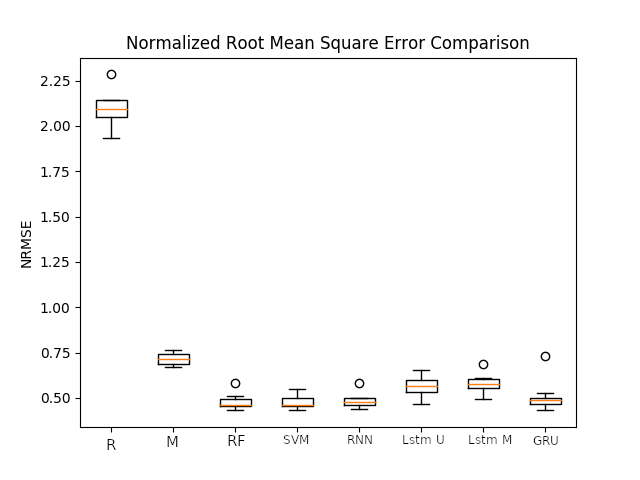
\includegraphics[width=9.5cm,keepaspectratio]{NrmseEditado.png}
     \caption{BoxPlot do NRMSE de cada modelo}
     \label{fig:BoxPlot NRMSE}
\end{figure}

\begin{figure}[!htb]
     \centering
     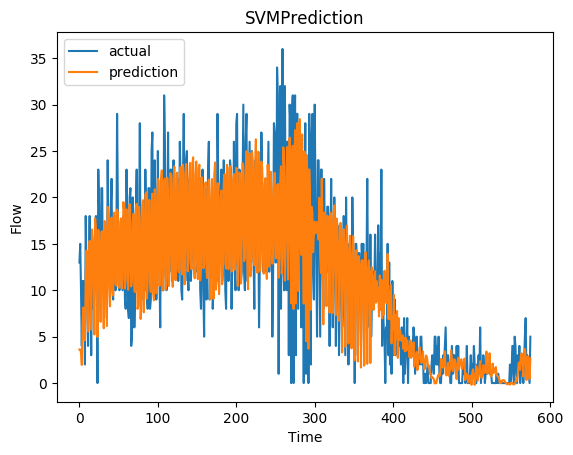
\includegraphics[width=9.5cm,keepaspectratio]{svm.png}
     \caption{Predição da SVM}
     \label{fig:pred_svm}
\end{figure}

\section{Conclusão}

Os resultados atuais indicam que os modelos utilizados são superiores as bases de comparação. Porém os resultados mostrados foram para modelos que ainda não passaram pela escolha de parâmetros e hiper-parâmetros, ou seja, ainda é possível melhorar os modelos. Deixando aberto ainda espaço para a melhora dos modelos.

Esse trabalho ainda está em andamento, futuramente serão realizadas as etapas abaixo:

\begin{itemize}
    \item Escolha dos parâmetros e hiper-parâmetros
    \item Implementação e comparação de todos os modelos com dados multi-variados
    \item Implementação e comparação de todos os modelos com dados de múltiplos sensores
\end{itemize}

\section{Agradecimentos}

Agradecemos os orientadores Li Weigang e Geraldo Filho e o professor Luis Garcia pela colaboração nesse projeto. Além disso, agradecemos ao DETRAN e Fábio Borges por nos fornecer os dados utilizados no trabalho.

\begin{thebibliography}{00}
\bibitem{b1} G. Eason, B. Noble, and I. N. Sneddon, ``On certain integrals of Lipschitz-Hankel type involving products of Bessel functions,'' Phil. Trans. Roy. Soc. London, vol. A247, pp. 529--551, April 1955.

\bibitem{b2} Zainab Abbas , Ahmad Al-Shishtawy , Sarunas Girdzijauskas  , Vladimir Vlassov, ``Short-Term Traffic Prediction Using Long Short-Term Memory Neural Networks,'' vol.2018 IEEE International Congress on Big Data.

\bibitem{b3} Yong-Ju Lee, OkGee Min ``Long Short-Term Memory Recurrent Neural Network
for Urban Traffic Prediction: A Case Study of Seoul,'' 2018 21st International Conference on Intelligent Transportation Systems (ITSC)

\bibitem{b4} Yisheng Lv, Yanjie Duan, Wenwen Kang, Zhengxi Li, Fei-Yue Wang ``Traffic Flow Prediction With Big Data: A Deep
Learning Approach,'' IEEE TRANSACTIONS ON INTELLIGENT TRANSPORTATION SYSTEMS, VOL. 16, NO. 2, APRIL 2015

\bibitem{b5} Simon Oh, Young-Ji Byon, Kitae Jang, Hwasoo Yeo, ``Short-term Travel-time Prediction on Highway: A Review of the Data-driven Approach,'' 2015 Transport Reviews, vol. 35, pp. 4-32

\bibitem{b6} Babcock, B.; Babu, S.; Datar, M.; Motwani, R.; Widom, J. Models and issues in data stream systems. In: Proceedings of the twenty-first ACM SIGMOD-SIGACT- SIGART symposium on Principles of database systems, New York, NY, USA: ACM, 2002, p. 1–16.

\bibitem{b7} Relatório  da  frota  circulante, ``https://www.sindipecas.org.br/sindinews/
Economia/2019/RelatorioFrotaCirculante\_Maio\_2019.pdf''


\end{thebibliography}
\end{document}